\documentclass[fontsize=12pt,		% Font size
			   toc=listof,			% List of... into table of contents % listofnumbered
			   paper=A4,			% A4 paper
			   headinclude=true,	% Include header into type area calculation
			   footinclude=false,	% Don't include footer into type area calculation
			   headsepline=true,	% Separating line between header and text
			   footsepline=false,	% Separating line between footer and text
			   DIV=calc,			% Auomatically calculate DIV
			   %BCOR=15mm,			% Binding correction
			   %twosided=true,
			   %open=right
			  ]{scrartcl}

\usepackage[english,ngerman]{babel}
\usepackage[utf8]{inputenc}
\usepackage[T1]{fontenc}

\usepackage{lmodern}
\usepackage{microtype}

\usepackage{textcomp}				% Avoids conflicts between siunitx and microtype
\usepackage{siunitx}				% Allow for german decimals, e.g. 1,344 instead of 1.344 + other stuff

\usepackage{graphicx}
\usepackage{listings}
\usepackage{color}
\usepackage{hyperref}

% Autorenangabe
\newcommand\mychapter[2]{\chapter{#2}\vspace{-1.5em}\hspace{2.1em}\emph{#1}\vspace{1.5em}}
\newcommand\mysection[2]{\section{#2}\vspace{-0.9em}\hspace{2.1em}\emph{#1}\vspace{1.5em}}
\newcommand\mysubsection[2]{\subsection{#2}\vspace{-0.5em}\hspace{3.2em}\emph{#1}\vspace{1.3em}}

% ToDO

\newcommand\todo[1]{\footnote{\textcolor{red}{\textbf{#1}}}}

% PDF Metadaten

\pdfinfo{
 /Title (BlinkenTiles)
 /Author (Fabian Gärtner, Sarah Häfele, Alexander Scheurer, Linda Schey, Johannes Winter, Meike Zöckler)
}

\begin{document}

%%%%%%%%%%%%%%%%%%%%%%%%%%%%%%%%%%%%%%%%%
% University Assignment Title Page 
% LaTeX Template
% Version 1.0 (27/12/12)
%
% This template has been downloaded from:
% http://www.LaTeXTemplates.com
%
% Original author:
% WikiBooks (http://en.wikibooks.org/wiki/LaTeX/Title_Creation)
%
% License:
% CC BY-NC-SA 3.0 (http://creativecommons.org/licenses/by-nc-sa/3.0/)
% 
% Instructions for using this template:
% This title page is capable of being compiled as is. This is not useful for 
% including it in another document. To do this, you have two options: 
%
% 1) Copy/paste everything between \begin{document} and \end{document} 
% starting at \begin{titlepage} and paste this into another LaTeX file where you 
% want your title page.
% OR
% 2) Remove everything outside the \begin{titlepage} and \end{titlepage} and 
% move this file to the same directory as the LaTeX file you wish to add it to. 
% Then add \input{./title_page_1.tex} to your LaTeX file where you want your
% title page.
%
%%%%%%%%%%%%%%%%%%%%%%%%%%%%%%%%%%%%%%%%%

%----------------------------------------------------------------------------------------
%	PACKAGES AND OTHER DOCUMENT CONFIGURATIONS
%----------------------------------------------------------------------------------------

%\documentclass[12pt]{article}

%\begin{document}

\begin{titlepage}

\newcommand{\HRule}{\rule{\linewidth}{0.5mm}} % Defines a new command for the horizontal lines, change thickness here

\center % Center everything on the page
 
%----------------------------------------------------------------------------------------
%	HEADING SECTIONS
%----------------------------------------------------------------------------------------

\Large Hochschule Furtwangen - Fakultät Digitale Medien\\[0.5cm] % Name of your university/college
{\Large \bfseries Interaktionsdesign}\\[0.5cm] % Major heading such as course name
\large Wintersemester 2014/15\\[0.5cm] % Minor heading such as course title

%----------------------------------------------------------------------------------------
%	TITLE SECTION
%----------------------------------------------------------------------------------------

\HRule \\[0.2cm]
%{ \huge \bfseries BlinkenTiles}\\[0cm] % Title of your document

\includegraphics[width=0.5\textwidth]{images/logo_final}\\[-0.35cm]
\HRule \\[0.7cm]
 
%----------------------------------------------------------------------------------------
%	AUTHOR SECTION
%----------------------------------------------------------------------------------------

\begin{minipage}{0.55\textwidth}
\begin{flushleft} \large
%\emph{Authoren:}\\
Fabian Gärtner, MIM1\\
Sarah Häfele, MIM1\\
Alexander Scheurer, MIM1\\
Linda Schey, MIM2\\
Johannes Winter, DIM1\\
Maike Zöckler, DIM1\\

\end{flushleft}
\end{minipage}
~
\begin{minipage}{0.4\textwidth}
\begin{flushright} \large
%\emph{Supervisor:} \\
Prof. Patricia Stolz\\
Prof. Dr. Matthias Wölfel\\ % Supervisor's Name
\end{flushright}
\end{minipage}\\[2cm]

% If you don't want a supervisor, uncomment the two lines below and remove the section above
%\Large \emph{Author:}\\
%John \textsc{Smith}\\[3cm] % Your name

%----------------------------------------------------------------------------------------
%	DATE SECTION
%----------------------------------------------------------------------------------------

{\large \today}\\[3cm] % Date, change the \today to a set date if you want to be precise

%----------------------------------------------------------------------------------------
%	LOGO SECTION
%----------------------------------------------------------------------------------------

%\includegraphics{Logo}\\[1cm] % Include a department/university logo - this will require the graphicx package
 
%----------------------------------------------------------------------------------------

\vfill % Fill the rest of the page with whitespace

\end{titlepage}
%\end{document}

\section*{Abstract}
Die vorliegende Arbeit stellt die Dokumentation zur Konzeption und prototypischen Umsetzung von \emph{BlinkenTiles} dar. BlinkenTiles ist eine großflächige Installation, die es Personen erlaubt, durch eine auf den Boden projizierte Sound-Matrix und durch das Tracking einer Microsoft Kinect mit dem eigenen Körper Musik zu machen. Die Installation wurde im Rahmen der Veranstaltung \textit{Interaktionsdesign} in den Masterstudiengängen \textit{Design Interaktiver Medien} sowie \textit{Medieninformatik} an der Fakultät Digitale Medien der Hochschule Furtwangen im Wintersemester 2014/2015 unter der Betreuung von Frau Prof. Stolz und Herrn Prof. Dr. Wölfel entwickelt.

\tableofcontents
\clearpage

%Bitte im folgenden \includes{} nutzen!


\section{Grundidee}
\subsection{Ideenfindung}
\subsection{Zielsetzung}
\subsection{Werbebotschaft}
\subsection{Strategische Planung}

\section{Planung und Skizzierung}
\subsection{Zielgruppenanalyse}
\subsection{Tests}
\subsection{Technischer Aufbau}

\section{Umsetzung des Prototypen}
\subsection{Modell Aufbau}
\newpage
\subsection{DMX-Scheinwerfer}
\mysubsection{Linda Schey}{Multimonitor Support}

Zu Beginn des Projektes wurde versuch eine möglichst große Projektionsfläche zu erhalten. In Ermangelung eines Beamers, der die gewünschte Größe projizieren konnte wurde auf drei Beamer zurückgegriffen, die dann nebeneinander ein jeder ein Drittel der Applikation darstellen sollte. Um dies zu realisieren musste aber das komplette Bild das projiziert werden sollte in drei einzelne Bilder geteilt werden. Da die Beamer nicht nebeneinander, sondern über einander aufgebaut werden sollten, damit das komplette Bild hoch und breit genug ist müssen die erhaltenen Bilder jeweils um 90° gedreht werden. Dafür wurde in Unity eine extra Kamera in die Szene eingefügt, die die Szene als RenderTexture aufnimmt. Diese RenderTexture wurde dann in drei einzelne Texturen getrennt. Jede Textur um 90° gedreht und dann nebeneinander als Gui-Elemente dargestellt. Soweit war diese Funktionalität auch schon implementiert, bis auf kleine Justierungen beim Zuschneiden der einzelnen Teil Texturen. \\
Ein anderer Ansatz war drei um 90° gedrehte Kameras in die Szene zu integreren die jeweils ein Drittel des Spielfeldes filmten. 
\begin{figure}[htbp]
	\centering
		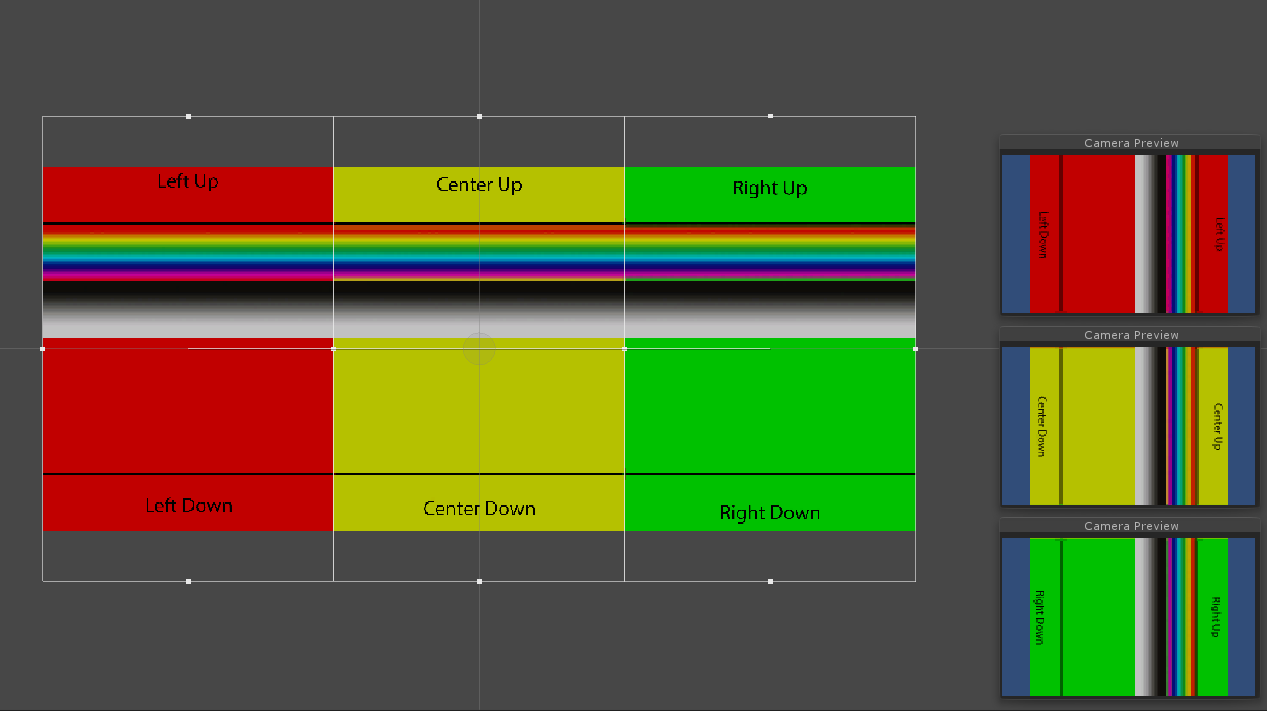
\includegraphics[width=0.8\textwidth]{images/RenderTextureBeispielSzene.PNG}
	\caption{Aufbau der Szene in Unity mit den drein RenderTextrure Ausschnitten am Beispiel eines Dummy Objektes}
	\label{fig:RenderTextureBeispielSzene}
\end{figure}
Daraus erhielt man drei RenderTextures, die dann nebeneinander als Gui rendern werden konnten. Dafür wurde zunächst mit einem Beispiel Objekt gearbeitet, das ein Material zugewiesen bekam, welches es bei der Entwicklung vereinfachte zu erkenne, ob die Kameras richtig ausgerichtet waren und dann auch entsprechend richtig auf die Gui gerendert wurden. 
\begin{figure}[htbp]
	\centering
		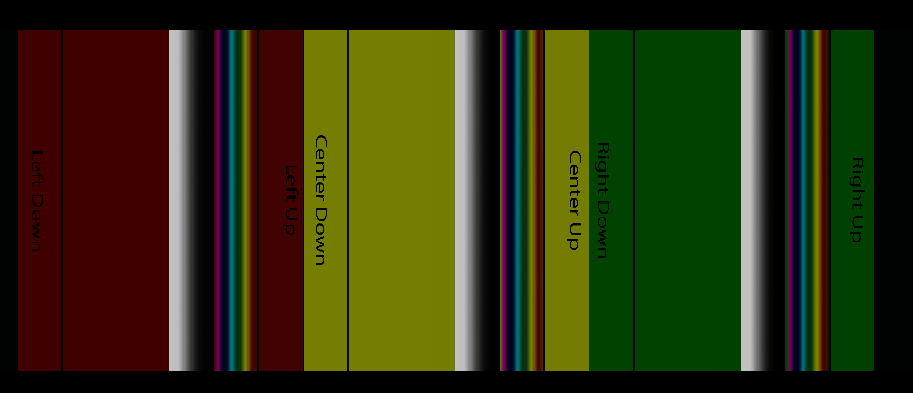
\includegraphics[width=0.8\textwidth]{images/RenderTexturesAlsGui.PNG}
	\caption{RenderTextures nebeneinander auf die Gui gerendert}
	\label{fig:RenderTexturesAlsGui}
\end{figure}\\
Die drei Kameras, mussten jedoch von Hand auf die Szene eingestellt werden, so dass es auch hier wieder zu Ungenauigkeiten hätte kommen können. Andererseits wäre man hier flexibler beim Ausrichten der Szene auf die drei Beamer gewesen, in dem man zum Beispiel die Übergänge zwischen den drei Texturen jeweils so hätte Platzieren können, dass sie auf einem Spalt der Felder des Spielfeldes gelegen wären. Auch dieser Ansatz wurde umgesetzt und hat mit funktioniert allerdings auch mit kleinen Ungenauigkeiten.\\
Beide Ansätze waren jedoch nicht zu 100 Prozent exakt,was das Aufteilten der Szene in drei Teil Texturen betraf. Außerdem standen keine drei identischen Beamer zur Verfügung, sodass es unter den einzelnen Beamern Unterschiede bei der Lichtintensität gab.
Da anstatt der Lösung mit den drei Beamern doch noch ein geeignetes Gerät gefunden wurde, das alleine die gewünschte Projektionsfläche erbrachte, wurde die Idee mit den drei Beamern, sowie die bisherige Implementierung dafür verworfen und ist im finalen Stand des Projektes nicht mehr enthalten.\\
\subsection{Tiles-Programmierung}
\subsection{Modi}
\subsection{Call to Action}
\subsection{Kinect-Erkennung}
\subsection{Audiogestaltung und Inspiration}
Das Konzept der Installation beruht auf einem klassischen Step-Sequenzer. Solche Sequenzer steuern die Klangerzeugung eines Synthesizers dahingehend, dass sowohl Rhythmus als auch Tonhöhe programmiert werden können. Der Name bezieht sich dabei auf die einzelnen „Steps“ die mit Tönen belegt werden können. Klassische analoge Step-Sequenzer wie der Roland TB 303 bieten 16 Schritte an, womit also pro Durchlauf 16 Töne gespielt werden können. Somit entspricht jeder Schritt einer 16tel Note eines Taktes. Es ist hervorzuheben, dass bei einem Step-Sequenzer die Noteneingabe nicht unmittelbar zu einer Klangerzeugung führt. Stattdessen tastet ein Impuls nacheinander alle „Steps“ ab und übermittelt die Daten an den Klangerzeuger. Nachdem der Impuls einmal durchgelaufen ist, beginnt der er wieder bei dem ersten Step. Dadurch entstehen repetitive Tonfolgen, sogenannte Loops. Step-Sequenzer haben gerade aufgrund dieser Beschränkung zahlreiche Genre wie Acid House, Electronic Body Music und Drum and Bass entscheidend geprägt.

Das Konzept der Installation weicht in mehreren Punkten vom klassischen Step-Sequenzer ab. Zum Einen gibt es statt 16 Schritten nur 8. Außerdem ist die Tonauswahl auf 5 Tonhöhen pro Schritt begrenzt. Des Weiteren wird ist ein Ton nur so lange aktiviert, wie auch eine Person auf dem entsprechenden Feld steht. Das musikalische Konzept berücksichtigt diese Einschränkungen. Da nur 5 Töne gespielt werden können und auch nur 8 Steps zur Verfügung stehen, wird ein Backing Track benötigt, der eine harmonische Grundlage für das Spiel des Instrumentes bietet.

Anspruch der Installation war es aber weniger ein komplexes Instrument zu bieten, viel mehr eine musikalische Spielwiese. Aus diesem Grund liegt die Entscheidung nahe, sich die technischen Beschränkungen zu Nutze zu machen. Es wurde also auf eine Skala zurückgegriffen, die einerseits nur 5 Töne hat und andererseits keine Halbtonschritte aufweist: die Anhemitonische Pentatonik. Der Vorteil liegt darin, dass keine kleinen Sekunden und Tritoni gespielt werden können, die für unsere Hörgewohnheiten „unrein“ klingen. Durch diese Maßnahme wurde also sichergestellt, dass unabhängig von Menge und Position der Benutzer ein recht harmonisches Gesamtbild entsteht, auch wenn dadurch auf die Leittonwirkung einer Diatonik oder Hemitonischen Pentatonik verzichtet werden muss. Außerdem war der Tonumfang natürlich auf eine Oktave beschränkt, mehr als 5 Tonhöhen hätten das musikalische Ergebnis interessanter gestaltet aber auch die Nutzerfreundlichkeit eingeschränkt. Da die Installation in erster Linie intuitiv bedienbar sein sollte, wurde der Tonumfang nicht weiter ausgebaut.

Für den experimentellen Modus der Installation wurden drei Backing Tracks mit jeweils 5 zugehörigen Tonhöhen vorproduziert. Der durchlaufende Impuls wurde auf die Geschwindigkeit des entsprechenden Backing Tracks angepasst und die zugehörigen Töne auf die Felder gemappt. Da der Klangerzeuger kein Synthesizer sondern ein Sampler war, mussten die Einzeltöne im Voraus synthetisiert und gerendert werden. Grundsätzlich wurden eher sphärische Klänge mit langem Nachhall (entweder Reverb oder Hüllkurvengenerator) eingesetzt, da die Benutzer der Installation keinen Einfluss auf die Länge des Tons hatten. In Hüllkurvenparametern gesprochen musste also der Attack deutlich hörbar sein um ein auditives Feedback zu geben, die Sustainlautstärke musste relativ schnell erreicht werden und wesentlich leiser als der Attack sein, damit sich bei mehreren Personen die Sounds nicht zu stark überdeckten. Dadurch wurden relativ perkussive Klänge erzeugt, die durch den Nachhall eine gewisse Stetigkeit erreichten. Die Backing Tracks bildeten das rhythmische und harmonische Grundgerüst und wurden ebenfalls im Voraus produziert und gerendert. Dabei wurde Wert darauf gelegt, zwar eine harmonische Orientierung zu bieten, der Backing Track sollte jedoch keine komplexe harmonische Struktur aufweisen. In den Backing Tracks wurde also ebenfalls weitgehend auf die oben erwähnte Pentatonik zurückgegriffen, um aber ein wenig musikalische Spannung zu kreieren, wurden an ausgewählten Stellen auch Töne aus diatonischen Skalen verwendet.

Für den Challenge Modus wurden ebenfalls drei Backing Tracks und passende Töne vorproduziert, da jedoch die technischen und konzeptionellen Bedingungen andere waren, soll darauf noch näher eingegangen werden. Das Ziel des Challenge Modus ist es, mit der Installation bekannte Lieder nachzuspielen, ähnlich wie bei Guitar Hero. Problematisch ist jedoch, dass die Reaktionsgeschwindigkeit der Benutzer nicht so schnell ist wie es eigentlich nötig wäre. Das größte Hindernis ist jedoch, dass die Nutzer die Installation verlassen müssen, wenn sie keinen Ton spielen wollen. Sobald sie auf irgendeinem Feld stehen und der Impuls dieses erreicht wird der Ton getriggert, auch wenn er falsch ist. Anders gesagt: Die Zustände der Nutzer auf dem Spielfeld sind analog, benötigt wären aber digitale Zustände, an oder aus. Aus diesem Grund mussten Songs gefunden werden, die einerseits recht bekannt sind, ein minimales Tonspektrum aufweisen und langsam genug sind um mit der Installation spielbar zu sein. Die Entscheidung fiel auf „Smoke on the water“ von Deep Purple, „Paint it black“ von den Rolling Stones und “One” von Swedish House Mafia.

Die Ausschnitte der Lieder die benutzt werden sollten, wurden zunächst nachgespielt und aufgenommen. Dabei war es wichtig, hervorstechende Klangeigenschaften der Originale zu berücksichtigen um den Wiedererkennungswert nicht zu verlieren. Bei „Smoke on the water“ wurde beispielsweise ein bekannter britischer Röhrenverstärker mit vorgeschaltetem Overdrive verwendet. Nachdem alle Einzelspuren aufgenommen waren musste bestimmt werden, welche Spuren den Backing Track bildeten und welche Spur von den Nutzern gespielt werden sollte. Der Backing Track wurde dann ohne die entsprechende Spur gerendert. Die Spur die der Nutzer spielen sollte, musste nun in kleine Samples geschnitten werden um auf die verschiedenen Felder aufgeteilt werden zu können.

\begin{figure}[htbp] 
  \centering
     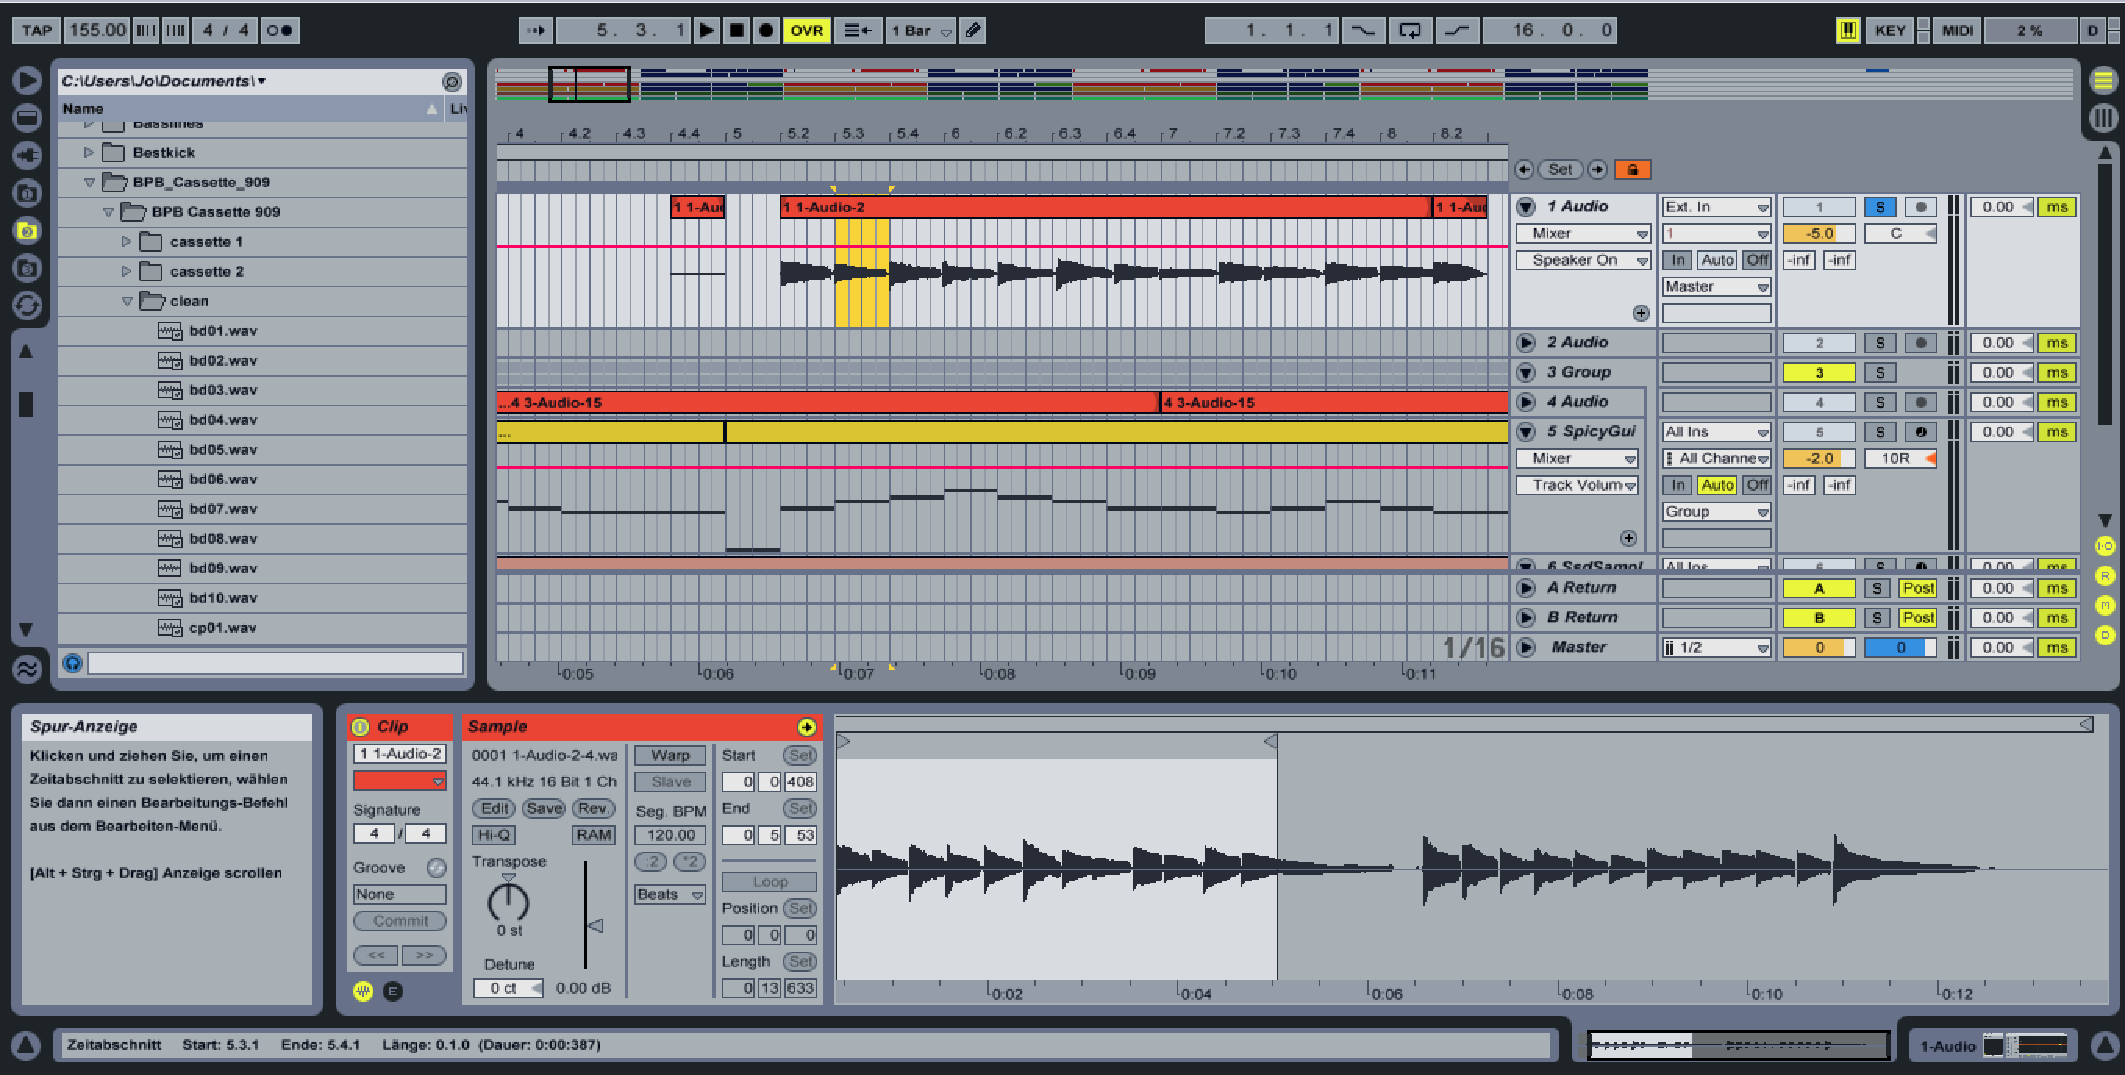
\includegraphics[width=0.9\textwidth]{images/Musikkonzeption}
  \caption{Schneiden der Spuren in Ableton Live}
  \label{fig:audio1}
\end{figure}

Dabei ergaben sich in einigen Fällen Probleme bezüglich der Tonlänge. Da die Schritte des Step-Sequenzers immer auf einen bestimmten Rhythmuswert quantisiert waren, zum Beispiel 8tel oder 16tel Noten, mussten hinsichtlich Synkopen oft Kompromisse eingegangen werden. Bei „One“ führte dies dazu, dass der Impuls so schnell war, dass das Lied damit praktisch unspielbar wurde. Für den Challenge Modus erwies sich damit das Konzept der Soundmatrix insgesamt als relativ ungeeignet, während im experimentellen Modus musikalisch interessante Ergebnisse erreicht wurden.

\section{Tag der Medien}
\subsection{kleiner Bericht mit Fotos}
\subsection{Praxiserfahrungen}

\section{Showreel}
\section{Fazit, mögl. Weiterentwicklungsmöglichkeiten}

\end{document}